\section{Einleitung}
\subsection{Einführung in die Thematik}
\blindtext\nomenclature{W3C}{World Wide Web Consortium}
\blindtext\footcite[Vgl. ][]{mswpf}\footcite[Vgl. ][19]{sadtler_rechtskonformes_2017}

\subsection{Problemstellung und Zielsetzung}
\blindtext

\subsection{Methodischer Aufbau der Arbeit}
\blindtext

\section{Hauptteil}
\subsection{Grundlagen der Wirtschaftsinformatik}
„Dies ist ein direktes Zitat."\footcite[][224]{mertens_digitalisierung_2017} \blindtext\footcite[Vgl. ][]{msdatabind}\footcite[Vgl. ][]{lambda}\footcite[Vgl. ][34]{Digitaloekonomie}
\blindenumerate
\blindtext\footcite[Vgl. ][415-426]{Tanenbaum2016}\footcite[Vgl. ][223]{mandl_internet_2019}

\begin{figure}[!htb]
    \caption{Terminal}
    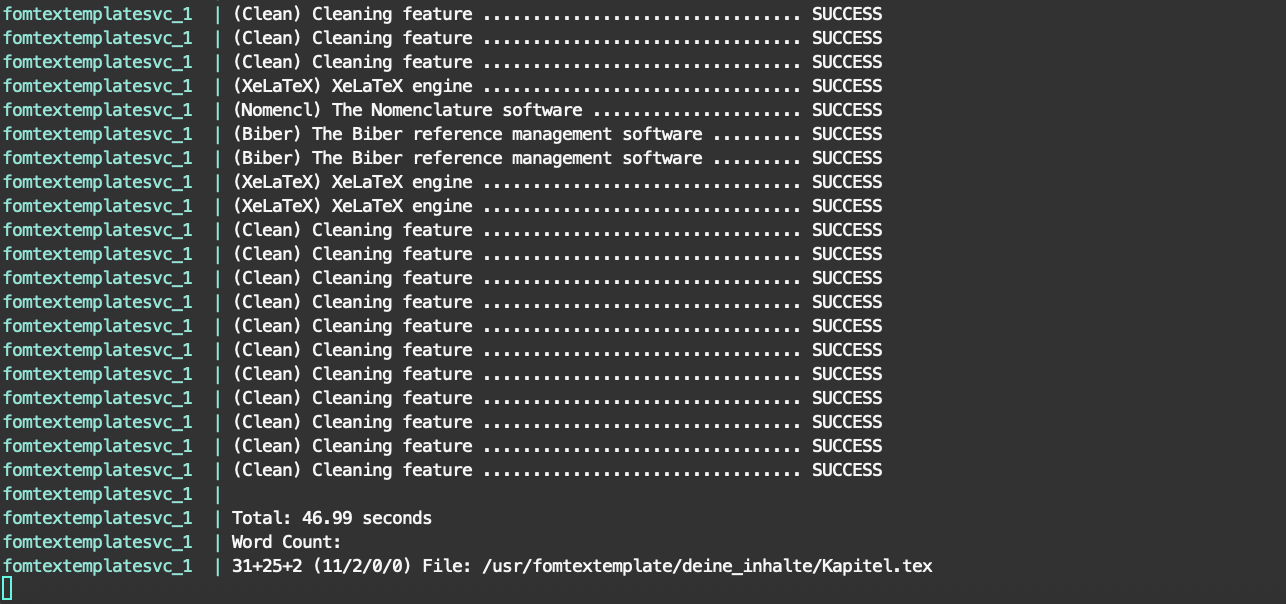
\includegraphics[width=1\textwidth]{.github/terminal}
    \captionsetup{width=1\textwidth}
    \capquelle{\cite[][200]{bsp}}\label{abb_bsp}
\end{figure}
\blindtext

\subsubsection{Design-Prinzip der Separierung von Verantwortlichkeiten}
\blindtext\footcite[Vgl. ][79]{Schelinski2019}

\begin{table}[!htb]\label{tabelle_eins}
    \setlength{\arrayrulewidth}{1pt}
    \begin{threeparttable}
        \caption{Tabelle Eins}
        \begin{tabularx}{\textwidth}[htb!]{|X|X|X|X|X|}
            \hline
            Spalte 1 & Spalte 2 & Spalte 3 & Spalte 4 & Spalte 5\\ \hline
            1 & 2 & 3 & 4 & Vivamus nunc nunc, molestie ut, ultricies vel, semper in, velit. \\ \hline
            1 & 2 & 3 & 4 & Vivamus nunc nunc, molestie ut, ultricies vel, semper in, velit. \\ \hline 
            1 & 2 & 3 & 4 & Vivamus nunc nunc, molestie ut, ultricies vel, semper in, velit. \\ \hline 
            1 & 2 & 3 & 4 & Vivamus nunc nunc, molestie ut, ultricies vel, semper in, velit. \\ \hline 
        \end{tabularx}
        \begin{tablenotes}[flushleft]
            \item \normalsize{Quelle: \cite[][207]{bsp}}
        \end{tablenotes}
    \end{threeparttable}
\end{table}

\Blindtext\footcite[Vgl. ][34]{Digitaloekonomie}\footcite[Vgl. ][]{mesh}
\blinditemize
\blindtext\footcite[Vgl. ][511]{Tanenbaum2016}

\subsubsection{LaTeX-Befehle}
    \textnormal{Normale Schrift} 
    \textbullet\addspace \textbf{fette Schrift} 
    \textbullet\addspace \textit{kursive Schrift} 
    \textbullet\addspace \textsl{schiefe Schrift} 
    \textbullet\addspace \underline{unterstrichen} 
    \textbullet\addspace \texttt{Schreib\-ma\-schi\-ne} 
    \textbullet\addspace \textsf{Sans Serif} 
    \textbullet\addspace \textrm{Roman} 

\subsection{Test: Silbentrennung - Gegenüberstellung - darf nicht in den weißen Rand laufen}
Im zweiten Kapitel wird zunächst der Begriff \textit{Bring Your Own Device} (BYOD) definiert. Darauffolgend wird dargelegt welche Fokusse gesetzt werden sollen und Schlussfolgerungen gezogen, sowie eine Sicherheitsrichtlinie abgeleitet. Welche als Grundlage einer Gegenüberstellung mit etablierten Konzepten dient, sodass Strategien erörtert werden können. 

\section{Test der Ebenen}
\subsection{Ebene 2}
\blindtext
\subsection{Ebene 2.2}
\blindtext
\subsubsection{Ebene 3}
\blindtext
\subsubsection{Ebene 3.2}
\blindtext
\subsubsubsection{Ebene 4}
\blindtext
\subsubsubsection{Ebene 4.2}
\blindtext

\section{Schluss}
\subsection{Fazit}
\blindtext (vgl. Abbildung \ref{abb_bsp}).

\subsection{Ausblick}
\blindtext
